%\input{tcilatex}


\documentclass[notes=show, beamer, handout]{beamer}
%%%%%%%%%%%%%%%%%%%%%%%%%%%%%%%%%%%%%%%%%%%%%%%%%%%%%%%%%%%%%%%%%%%%%%%%%%%%%%%%%%%%%%%%%%%%%%%%%%%%%%%%%%%%%%%%%%%%%%%%%%%%%%%%%%%%%%%%%%%%%%%%%%%%%%%%%%%%%%%%%%%%%%%%%%%%%%%%%%%%%%%%%%%%%%%%%%%%%%%%%%%%%%%%%%%%%%%%%%%%%%%%%%%%%%%%%%%%%%%%%%%%%%%%%%%%
\usepackage{amssymb, amsthm}



\usepackage{amsmath}
\usepackage{graphicx}
\usepackage{epstopdf}
\usepackage{mathpazo}
\usepackage{hyperref}

%\usepackage[margin=0.5in]{geometry}

\usepackage{multimedia}
\usepackage{multirow, booktabs}

%
%\usepackage{tikz}
%\usetikzlibrary{pgfplots.groupplots, arrows, calc, arrows.meta, decorations.markings, math}
%\usepackage{pgfplots}
%\pgfplotsset{compat=1.13}
%\usepackage{fix-cm}

\graphicspath{{./figures/}}



\newtheorem{proposition}{Proposition}

\newcommand{\VaR}{{\text{VaR}}}
\newcommand{\ES}{{\text{ES}}}
\newcommand{\MS}{{\text{MS}}}
\newcommand{\TCM}{{\text{TCM}}}
\newcommand{\R}{{\mathbb{R}}}
\newcommand{\trho}{\tilde\rho}

\DeclareMathOperator*{\argmin}{arg\,min}
\newcommand{\PSet}{\mathcal{P}}
\newcommand{\X}{\mathcal{X}}
\newcommand{\LInf}{\mathcal{L}^{\infty}(\Omega, \mathcal{F}, P)}
\newcommand{\be}{\begin{equation}}
\newcommand{\ee}{\end{equation}}
\newcommand{\bee}{\begin{equation*}}
\newcommand{\eee}{\end{equation*}}

%\newtheorem{definition}{Definition}
\setcounter{MaxMatrixCols}{10}
%TCIDATA{OutputFilter=LATEX.DLL}
%TCIDATA{Version=5.50.0.2960}
%TCIDATA{<META NAME="SaveForMode" CONTENT="1">}
%TCIDATA{BibliographyScheme=Manual}
%TCIDATA{Created=Monday, March 27, 2006 16:48:17}
%TCIDATA{LastRevised=Saturday, December 15, 2012 17:35:51}
%TCIDATA{<META NAME="GraphicsSave" CONTENT="32">}
%TCIDATA{<META NAME="DocumentShell" CONTENT="Other Documents\SW\Slides - Beamer">}
%TCIDATA{Language=American English}
%TCIDATA{CSTFile=beamer.cst}

\newenvironment{stepenumerate}{\begin{enumerate}[<+->]}{\end{enumerate}}
\newenvironment{stepitemize}{\begin{itemize}[<+->]}{\end{itemize}}
\newenvironment{stepenumeratewithalert}{\begin{enumerate}[<+-| alert@+>]}{\end{enumerate}}
\newenvironment{stepitemizewithalert}{\begin{itemize}[<+-| alert@+>]}{\end{itemize}}
\usetheme{Madrid}
%\input{tcilatex}
%\begin{document}

\title[Designing Stable Coins]{Designing Stable Coins}

\author[S. Kou] % (optional, use only with lots of authors)
{Steven Kou\inst{1} }
% - Use the \inst{?} command only if the authors have different
%   affiliation.

\institute[NUS] % (optional, but mostly needed)
{
  \inst{1}
  Risk Management Institute and Department of Mathematics\\
  National University of Singapore \\
  Based on the paper by Yizhou Cao, Min Dai, Steven Kou, Lewei Li, and Chen Yang
}

\date{}
%\maketitle
%\tableofcontents

% Delete this, if you do not want the table of contents to pop up at
% the beginning of each subsection:

\AtBeginSection[] {
  \begin{frame}<beamer>
    \frametitle{Outline}
    \tableofcontents[currentsection]
  \end{frame}
}

\begin{document}

\begin{frame}
  \titlepage
%   \begin{center}
%School of Data Science
%
%
%Fudan University
%
%\end{center}
\end{frame}

\begin{frame}
  \frametitle{Outline}
  \tableofcontents
  % You might wish to add the option [pausesections]
\end{frame}

\section{Introduction to FinTech}

\begin{frame}
    \frametitle{Introduction}
    \begin{itemize}
        \item Fintech is a new word.  Fintech vs. Techfin
        \pause
        \item ``Fintech takes the original financial system and improves its technology. Techfin is to rebuild the system with technology.'' Jack Ma from Alibaba, {\it South China Morning Post}, Dec 2, 2016.
        \pause
        \item Neither IT issues nor philosophical issues will be discussed.
%           \item  For example, we will not discuss how to build an efficient money transfer and payment system via mobile devices; we will also not discuss why Fintech exists and whether Fintech is good or bad for the society.
%        \pause
%        \item ``A Theory'' not ``The Theory.''
        \pause
        \item Fintech = Quantitative Finance 2.0?
   \end{itemize}
\end{frame}

\begin{frame}
    \frametitle{A New Journal: Digital Finance}

    \begin{itemize}
        \item To be published by Springer.
    \item  Co-editors, Wolfgang Hardle from HU Berlin and myself
    \item Professors Min Dai and Ying Chen are in the editorial board.
   \item Subject fields:

    \begin{itemize}
       \item Cryptocurrencies
       \item Blockchain Technology
       \item Robo Advising
       \item Text Mining
       \item P2P Financing
       \item Financial Privacy Issues
        \item Digital Banking
       \item  Internet Finance
       \item Financial Inclusion
    \end{itemize}
       \end{itemize}
\end{frame}






\section{Background of Cryptocurrencies and Our Contribution}



\begin{frame}{Background}




\begin{itemize}
\item Bitcoin, ETH, and other cryptocurrencies---distributed payment systems
\begin{itemize}
\item A peer-to-peer network: A payment from one user to another is processed without any intermediary.
\item Blockchain: All transaction records are stored by every user.
\item Anonymous payment: Anonymous transaction orders are recorded to Blockchain, after miners' verification, and updated to all users immediately.
\end{itemize}
  \pause
  \item Benefits of using cryptocurrencies
\begin{itemize}
\item Low cost without intermediary
\item Easy to maintain the ledger inside the Blockchain system
\item Privacy
%\item Fast and less regulation.
\end{itemize}

%\item Miners play central role in the system
%\begin{itemize}
%\item Provide (verification and/or other) services and maintain the Blockchain records.
%\item Are compensated in two ways:
%\begin{itemize}
%\item Blockchain rewards (determined by the system);
%\item Transaction fees (determined by the market).
%\end{itemize}
%\end{itemize}

\end{itemize}
\end{frame}


%\begin{frame}{Bitcoin System}
%
%\begin{figure}
%\centering
%\includegraphics[width=0.85\linewidth]{./Figure_0830/Bitcoin_system_1}
%\label{fig:Bitcoin_system}
%\end{figure}
%%\tiny{Source: Authors}
%\end{frame}



%\begin{frame}{Some facts}
%\begin{itemize}
%\item Users' Demand:
%
%\item Miners and Money supply
%\item Holding distribution
%\item Volatility and bubbles
%\end{itemize}
%\end{frame}


%\begin{frame}{Controlled Supply of Bitcoin}
%\begin{itemize}
%\item Total number of Bitcoins: 21 million.
%\item The supply of Bitcoin ended on May 7th, 2140.
%\end{itemize}
%\begin{figure}
%\centering
%\includegraphics[width=8cm]{./Figure_0620/Bitcoin_supply_true_2}
%%\caption{}
%\label{fig:bitcoin_supply}
%\end{figure}
%\end{frame}


\begin{frame}{The Need for Stable Coins}

%\begin{itemize}

% \pause
%\item Bitcoin price has increased about 250,000 times from \$0.08 in July 2010 to about \$19,870 in Dec 2017, and then dropped to about \$7600 now.
%What will be the price of Bitcoin in the long run?
% \pause
%\item The need for stable coins
\begin{itemize}
\item Stable coins can be used within the Blockchain to settle payments.
\item Stable coins can be used in crypto money market accounts.
\item Stable coins can be used by miners, who may find that it is difficult to convert the mined coins into traditional currencies in some countries.
\item The existing cryptocurrencies are too volatile to be served as stable coins.
\end{itemize}
%\end{itemize}
\end{frame}


\begin{frame}{ETH Coin}

ETH/USD price data from 1 Oct 2017 to 28 Feb 2018. 

\begin{figure}[htb]
\begin{centering}
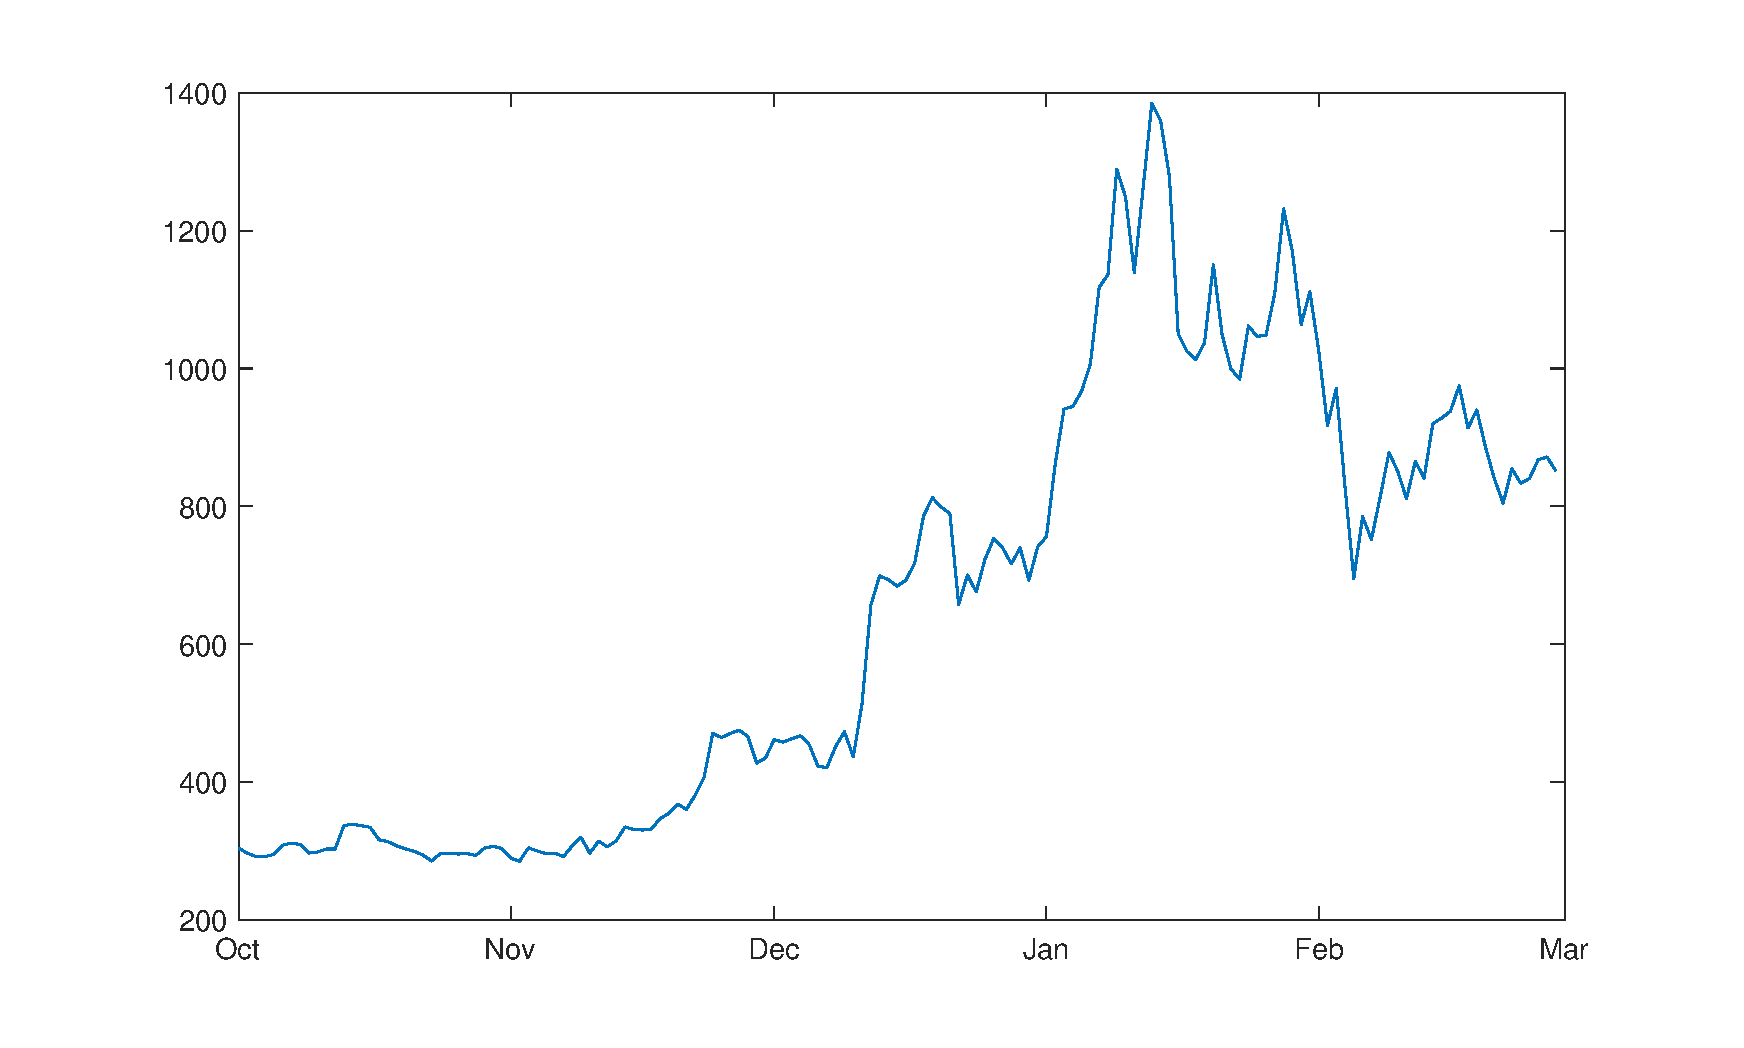
\includegraphics[width=0.95\textwidth]{eth_price}
\par\end{centering}
\caption{ETH/USD Price from 1 Oct 2017 to 28 Feb 2018}\label{fig:ethprice}
\end{figure}
\end{frame}


\begin{frame}{The Need for Stable Coins}

\begin{itemize}
\item How to create stable coins?
\pause
\item ``The Holy Grail of Cryptocurrency'' (Forbes, March 12, 2018, The Sydney Morning Herald, Feb 22, 2018, Yahoo Finance, Oct 14, 2017)
\pause
\item There are at least 3 existing ways to issue stable coins in Blockchain networks.
\end{itemize}
\end{frame}



\begin{frame}{Existing Stable Coins (1)}
\begin{itemize}
\item Issuance backed by accounts in cash, gold, oil, etc.: One has certain assets and issues tokens that represent a claim on the underlying asset.
\begin{itemize}
\item The most famous one is Tether,
which  100\% backed by USD. The conversion rate is 1 tether USDT equals 1 USD. Disadvantage: The total assets is about \$62.46 million, but the total liabilities is \$63.014 million, with a negative equity more than half million.
\item  Tokens are claimed to link to gold, although it is difficult to verify the claims, e.g. Digix, GoldMint, Royal Mint Gold, OzCoinGold, ONEGRAM.
\item Petro, issued by Venezuela and backed by one barrel of oil.
\end{itemize}
\end{itemize}
\end{frame}


\begin{frame}{Existing Stable Coins (2)}

\begin{itemize}
\item  Issuance backed by over-collateralized cryptocurrencies with automatic exogenous liquidation.
\begin{itemize}
\item For example, one can generate \$100 worth of stable coins by depositing \$150 worth of Ether. The collateral will be sold automatically by the smart contract, if the Ether price reaches \$110.
\item  Examples include token issued by BitShares and MakerDAO.
\end{itemize}
\end{itemize}
\end{frame}

\begin{frame}{Existing Stable Coins (3)}

\begin{itemize}
\item Automatic adjustment of the quantity of coin supply, called seigniorage shares.
\begin{itemize}
\item When the price is too high, new coins are issued. When the price is too low, bonds are issued to remove coins from circulation.
\item  Examples include Basecoin, etc.
\end{itemize}

\end{itemize}
\end{frame}

\begin{frame}{Government-Backed Stable Coins}

\begin{itemize}
\item Besides Venezuela, other countries are considering issuing cryptocurrencies, including Russia, China (Bloomberg news, Feb 13, 2018).
\item CAD-coin: Canadian government also did ``Project Japser'', in which a Blockchain network is built for domestic interbank payments settlement.
\item Fedcoin: There is a virtual currency working group under the Federal Reserve System in U.S. The Fedcoin is used internally. 
\item ``The goal is to create a stable (less price volatility) and dependable cryptocurrency that delivers the practical advantages of Bitcoin even if this means involving the central government and abandoning the Libertarian principles that many believe underlay Bitcoin’s creation.'' Rod Garrett (2016).
\end{itemize}

\end{frame}

\begin{frame}{Government Backed Stable Coins}





There are several advantages of issuing stable coins by governments
\begin{itemize}
\item They are cheaper to produce than the cash in bills or coins, and stable coins are never worn out.
\item They can be tracked and taxed automatically by the Blockchain technology.
\item They can facilitate statistical works, such as GDP calculation and collecting consumer data.
\item They cannot be forged (at least in theory).
\item They can simplify legal money transfers inside and outside Blockchains.
\end{itemize}

The first countries that adapt stable coins will likely see the inflow of money from people who want stable currencies on Blockchains.
\end{frame}



\begin{frame}{Our Contribution}
\begin{itemize}
\item Inspired by the dual purpose funds popular in the US and China,
we design, for the first time to our best knowledge, several dual-class structures that
offer entitlements to either fixed income stable coins (class A coins) pegged to a
traditional currency or leveraged investment opportunities (class B coins).
 \pause
\item Due to downward resets, a vanilla A coin behaves like a corporate bond with the collateral amount being reset automatically.
 \pause
\item The vanilla A coin can be further split into additional coins, A' and B' or A0 and A1, to reduce volatility.
 \pause
\item Unlike traditional currencies, these new class A coins record all transactions on a blockchain
without centralized counter parties.
 \pause
\item By using the option pricing theory, we show that
proposed stable coins indeed have very low volatility; indeed the volatility of  A' and A0 are similar to that of the short
term U.S. treasury bonds.
\end{itemize}
\end{frame}

\begin{frame}{Practical Usages}
\begin{itemize}
\item The design of stable coins can be used alone in most cases, except in the case of Black Swan events, when the underlying cryptocurrency suddenly drops close to zero within an extremely short time period.
\item This is like the top tranche of a CDO contract. If the correlation of all firms covered within the CDO are close to 1, then one firm defaults leads to almost all other firms default.
\item To be truly stable, stable coins need a guarantee in the Black Swan events.
\item When combined with insurance from a government, similar to FDIC insurance, the design can also serve as a basis for issuing a sovereign cryptocurrency via a private-public partnership.
\item By doing so, the government can let the private sector do the job of issuing stable coins, except to provide insurance in rare cases, saving government human and financial resources.
\end{itemize}
\end{frame}

\section{Design Details}


\subsection{Vanilla A  and B Coins}

\begin{frame}{Vanilla A Coin, Overview}

\begin{itemize}
\item The dual-purpose funds with dividend payments in U.S. were investigated both theoretically and empirically in
Ingersoll (1976), Jarrow and O'Hara (1989), and Adams and Clunie (2006).
\begin{itemize}
\item Finite time horizon, no resets.
\item Standard Black-Scholes PDE.
\end{itemize}
\item China dual-purpose funds with fixed income payments, A and B shares (Dai, Kou, Yang and Ye (2017)).
\begin{itemize}
\item Infinite time horizon, upward and downward resets cause changes of the prices of the underlying asset, but not the exchange ratio of the shares.
\item Periodic PDE with nonlocal terminal and boundary conditions, time dependent lower boundary and time independent upper boundary.
\end{itemize}

\item Our vanilla A and B coins:
\begin{itemize}
\item Infinite time horizon,  upward and downward resets cause changes of the exchange ratio of the shares, but not the prices of the underlying asset.
\item Periodic PDE with nonlocal terminal and boundary conditions, time dependent lower boundary and time {\it dependent} upper boundary.
\end{itemize}
\end{itemize}

\end{frame}



\begin{frame}{Vanilla A Coin, Initial Split}

\begin{figure}
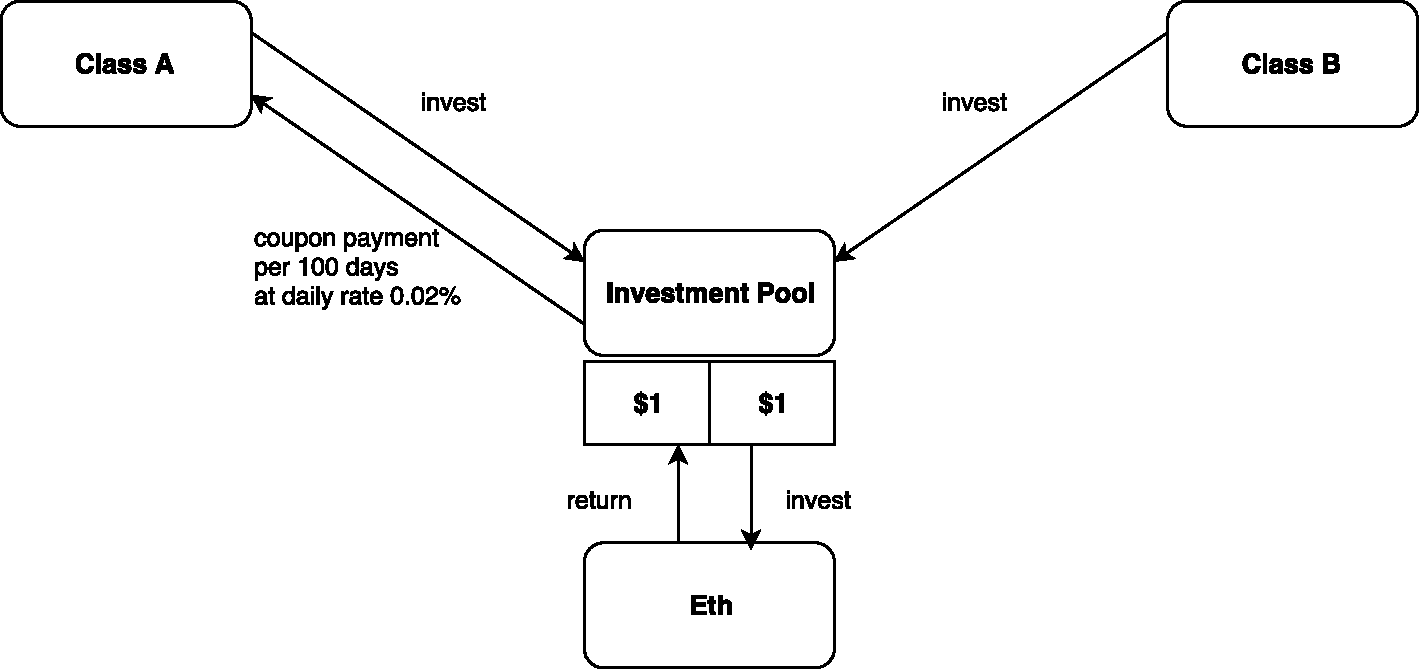
\includegraphics[width=\textwidth]{initial.pdf}
\caption{\footnotesize Initial Split. At the beginning, one share of Class A and B each invests \$1 in Eth. The Eth price is \$500, so two shares of Eth correspond to 500 shares of Class A coins and 500 shares of Class B coins. $\beta=1$.}
\end{figure}
\end{frame}

\begin{frame}{Vanilla A Coin, Regular Payout}
\begin{figure}
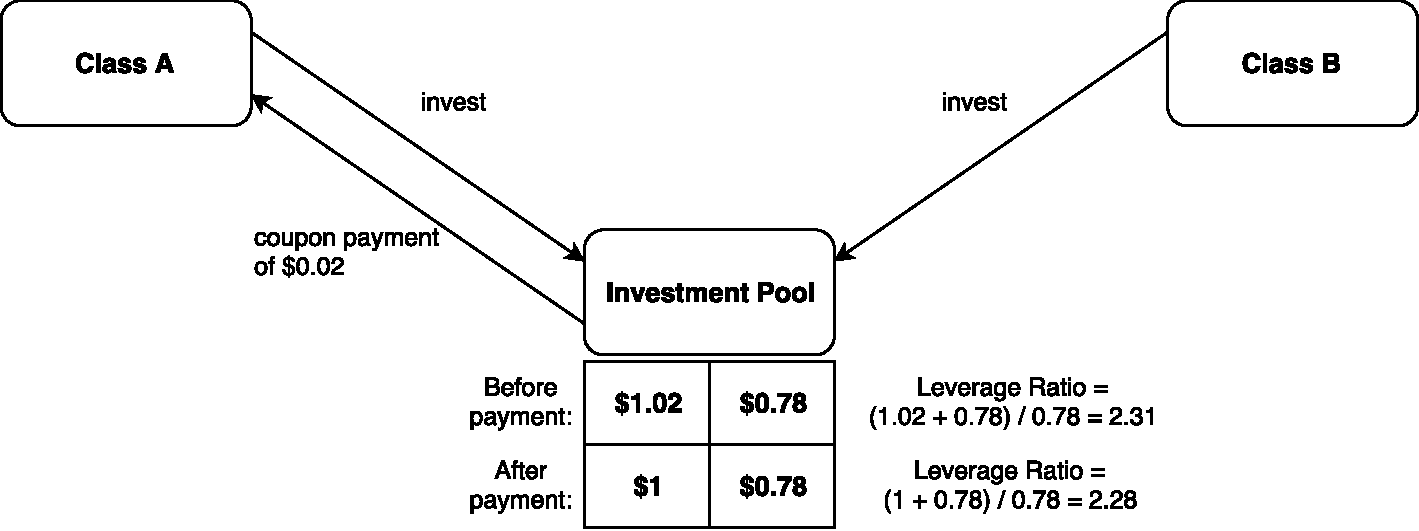
\includegraphics[width=\textwidth]{periodic.pdf}
\caption{\footnotesize Regular payout. After 100 days, the Eth price drops to \$450, so that total investment of one Class A coin and one Class B coin becomes \$1.8, within which \$1.02 belongs to Class A. A regular payout takes place, and Class A receives \$0.02 coupon payment. New exchange ratio: 2 shares of Eth now correspond to 505.62 ($=500\times\frac{2\times450}{2\times450-500*0.02}$) shares of Class A and 505.62 shares of Class B, yielding $\beta=1.01$. }
\end{figure}
\end{frame}


\begin{frame}{Vanilla A Coin, Upward Reset}

\begin{figure}
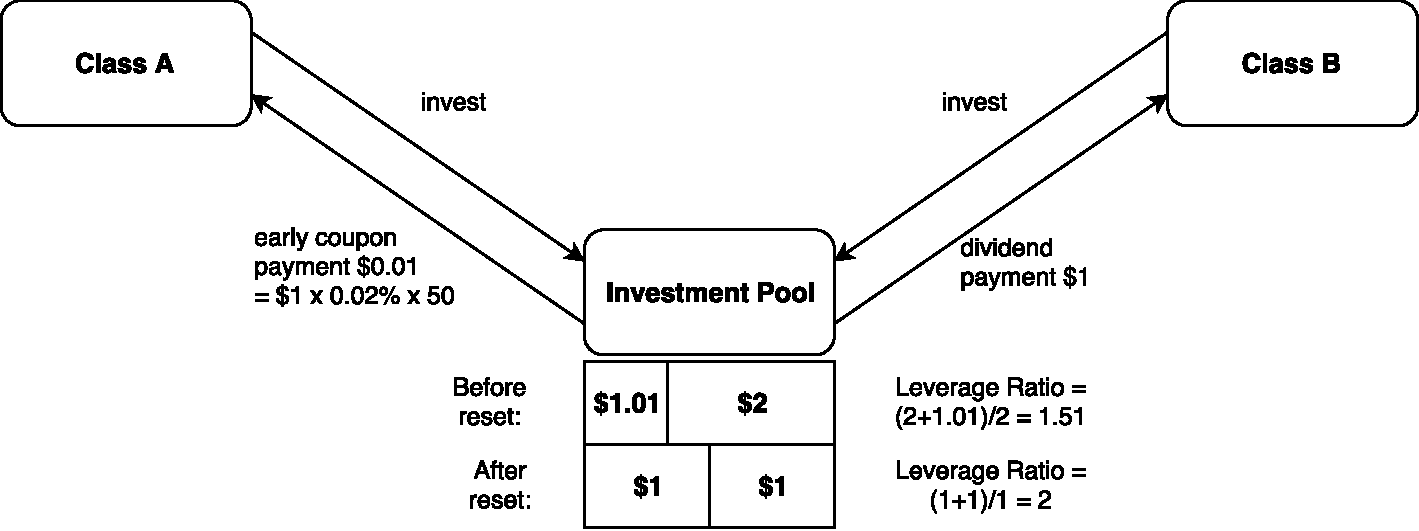
\includegraphics[width=\textwidth]{upward.pdf}
\caption{\footnotesize Upward Reset. After 50 days, the Eth price grows to \$760.95, and Class B NAV grows to \$2, triggering an upward reset. Class A NAV equals \$1.01, where \$0.01 is half-year accrued coupon. On this date, Class A receives \$0.01 coupon payment, and Class B receives \$1 dividend payment. New exchange ratio: 2 shares of Eth now correspond to 760.95 shares of Class A and 760.95 shares of Class B, yielding $\beta=1$. }
\end{figure}

\end{frame}


\begin{frame}{Vanilla A Coin, Downward Reset}


\begin{figure}
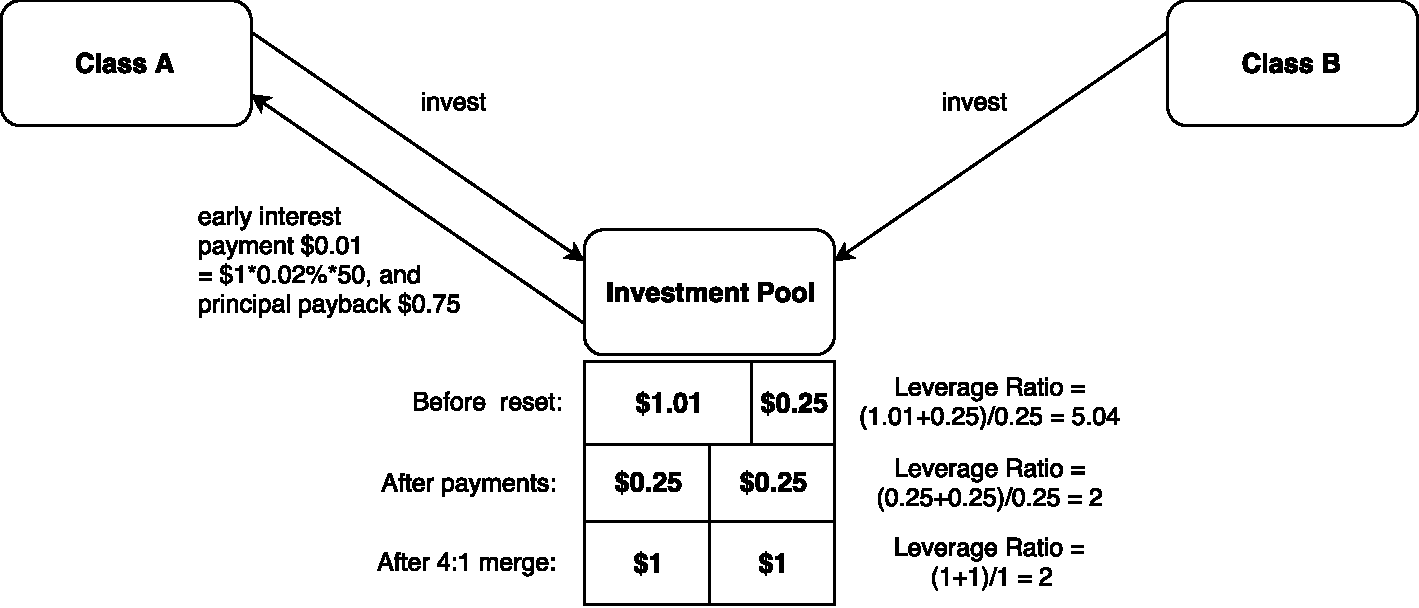
\includegraphics[width=\textwidth]{downward.pdf}
\caption{\footnotesize Downward Reset. After another 50 days, the Eth price drops to \$479.40, and Class B NAV drops to \$0.25, triggering an downward reset. Again, Class A NAV equals \$1.01, where \$0.01 is half-year accrued coupon. On this date, Class A receives \$0.01 coupon payment, as well as \$0.75 principal payback. Then, Class A and B each undergo a 4:1 merger, so that both have NAV equal to \$1. New exchange ratio: 2 shares of Eth now correspond to 479.40 shares of Class A and 479.40 shares of Class B, yielding $\beta=1$.}
\end{figure}

\end{frame}

\begin{frame}{Remarks}

\begin{itemize}
  \small
\item No arbitrage implies that
$$W_A^t +W_B^t=2 P_t/(\beta_t P_0),$$
where $P_t$ is the price of the underlying cryptocurrency, $W_A$ and $W_B$ are the price of the Class A and B coins, and $\beta_t$ is the conversion ratio, initially equal to 1, and will be changed on regular reset.
\item Coin A behaves like a corporate bond.
\begin{itemize}
\item Although Class A has a fixed coupon rate and its coupon payment is periodic and protected by the resets, its value is still volatile on non-coupon dates.
%\item This should be compared to the behavior of a corporate bond, whose value is influenced by its issuer's credit risk.
\item The main risk of Class A is not credit risk, but the risk of a downward reset. On a downward reset, a portion of Class A coin will be liquidated, so the investor will lose the value of future coupons that would be generated from this portion.
\item Therefore, a downward reset will reduce the value of Class A.
\end{itemize}
\item We propose two classes of more stable coins, the class of A' and B' coins and the class of A0 and A1 coins.
\end{itemize}
\end{frame}

\subsection{A' and B' Coins}


\begin{frame}{Overview of A' and B'}

\begin{itemize}
\item This second extension splits Class A into two sub-classes: Class A' and B'.
\item Class A' and B' invest in Class A coin.
\item At any time, two Class A coins can be split into one Class A' and one Class B' coin. Conversely, one Class A' and B' coin can be merged into 2 Class A coins.
\item Class B' borrow money from Class A' at the rate $R'$ to invest in Class A. 
%More precisely, the net asset value of Class A' is defined as $V_{A^\prime}=1+R^\prime t$, where $t$ is the time since last reset, and the net asset value of Class B' is defined as $V_{B^\prime}=1+2Rt-R^\prime t$.
\item $R'$ is set to close to the risk-free rate $r$, where the rate $R$ for Class A is generally much higher.
\item Class A' and B' resets {\it when and only when} Class A resets and Class A gets regular payout.
\item A' behaves like cash, except in extreme case, when the underlying asset suddenly jumps (not smooth transit) to close to zero.
\end{itemize}

\end{frame}


\begin{frame}{A' Coin, Regular Payout}

\begin{figure}
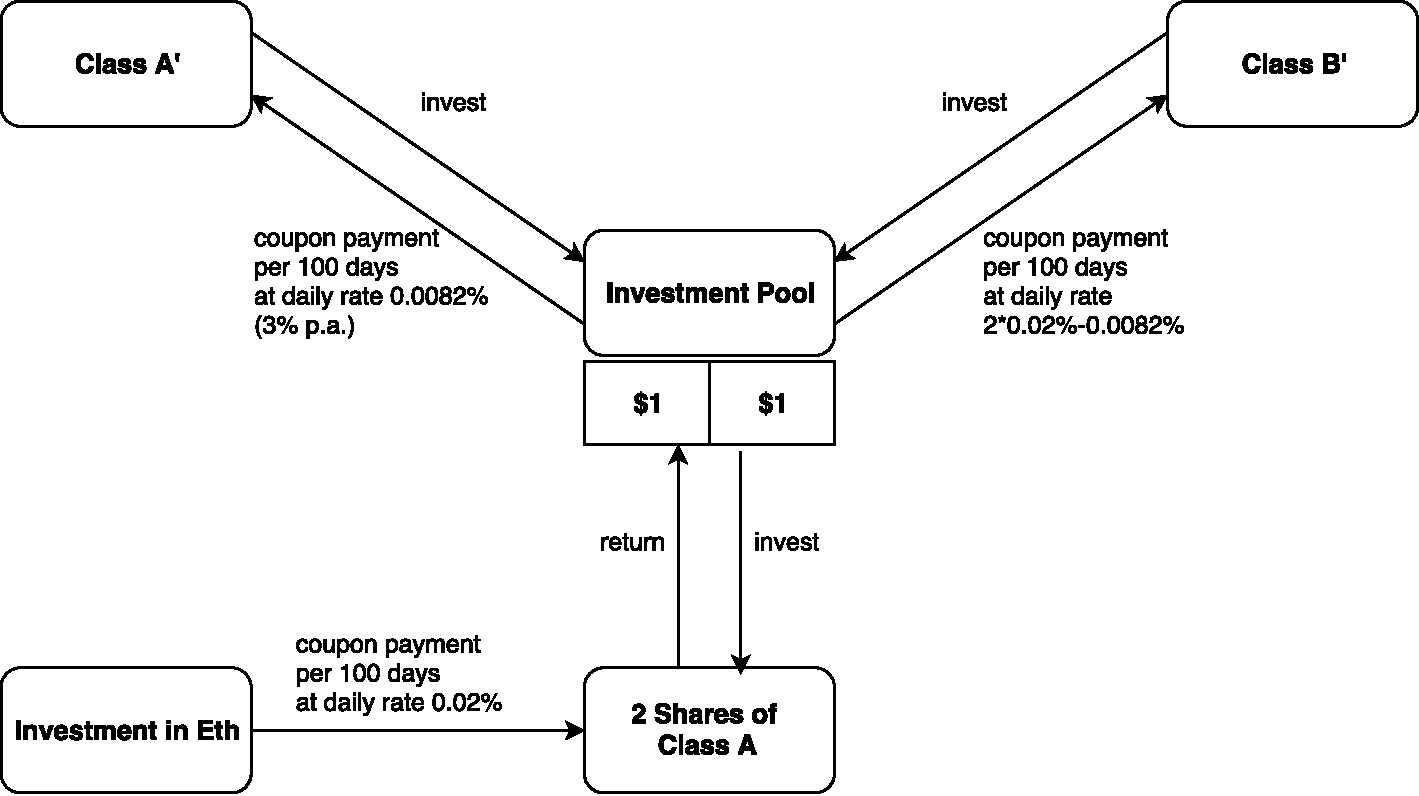
\includegraphics[width=\textwidth]{Ap_periodic.pdf}
\caption{\footnotesize What happens to A' on a regular payout date of A. On regular payout dates for A  (per 100 days), 2 shares of  A receives coupon payment \$0.04, i.e. at daily rate 0.02\%.}
\end{figure}

\end{frame}

\begin{frame}{A' Coin, Upward Reset}

\begin{figure}
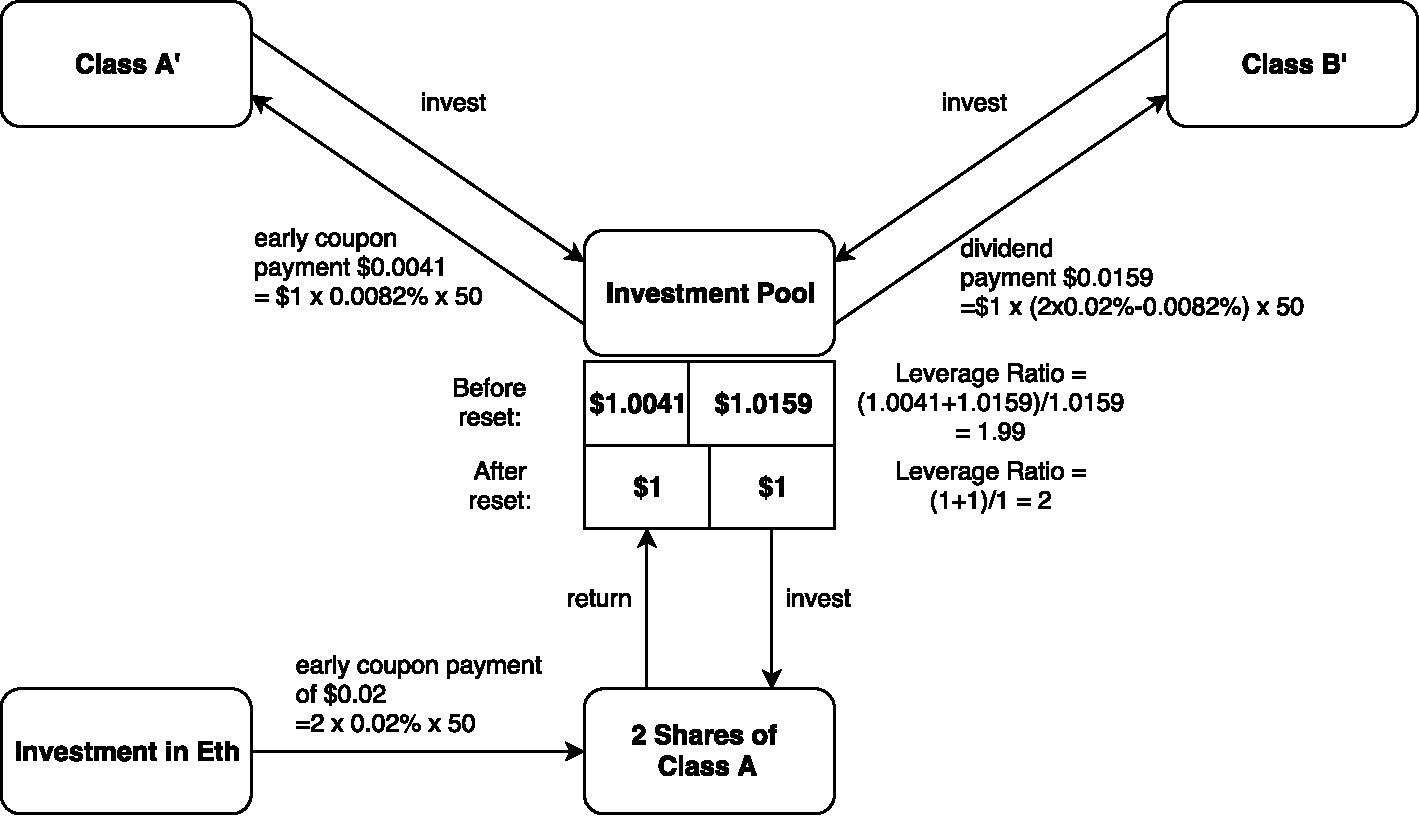
\includegraphics[width=\textwidth]{Ap_upward.pdf}
\caption{\footnotesize Upward Reset of Class A$^\prime$. After 50 days, Class B's NAV grows to \$2, triggering an upward reset.}
\end{figure}

\end{frame}


\begin{frame}{A' Coin, Downward Reset}

\begin{figure}
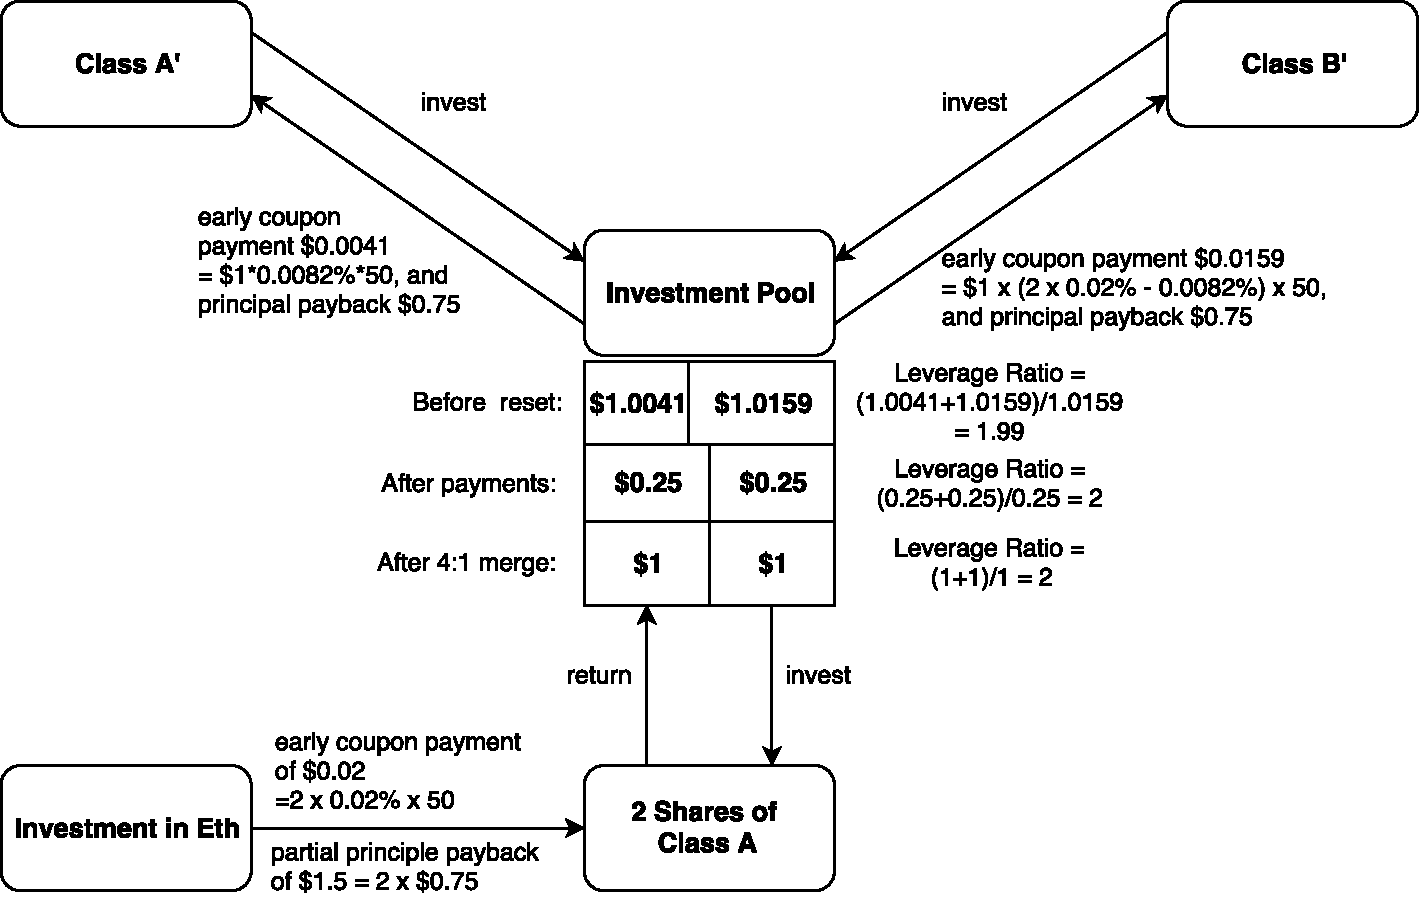
\includegraphics[width=0.85\textwidth]{Ap_downward.pdf}
\caption{\footnotesize After another 50 days, Class B NAV drops to \$0.25, triggering an downward reset.}
\end{figure}

\end{frame}


\subsection{A0 and A1 Coins}

\begin{frame}{Overview of A0 and A1}

\begin{itemize}

\item Each Class A coin is split into one Class A0 coin and one Class A1 coin.
\item On the next coupon payment date or reset date $t$, Class A1 receives the coupon payment for Class A, and then Class A1 is terminated.
\item Class A0 is then split into Class A0 coin and Class A1 coin, until the next reset when Class A1 receives payment and A0 is split again, so on and so forth.
%\item Note that when $V_B^{t-}\ge 1$, Class A0 does not receive any underlying coin and maintains the same quantity.
\item  At any time, the quantity of Class A0 and A1 maintains 1:1.
\item At any time, the value of Class A1 equals the expected discounted value of Class A's next payment on the next reset or coupon payment date.
\item The value of Class A0 equals the difference between values of Class A and A1.


\end{itemize}

\end{frame}


\begin{frame}{A0 Coin, Regular Payout}

\begin{figure}
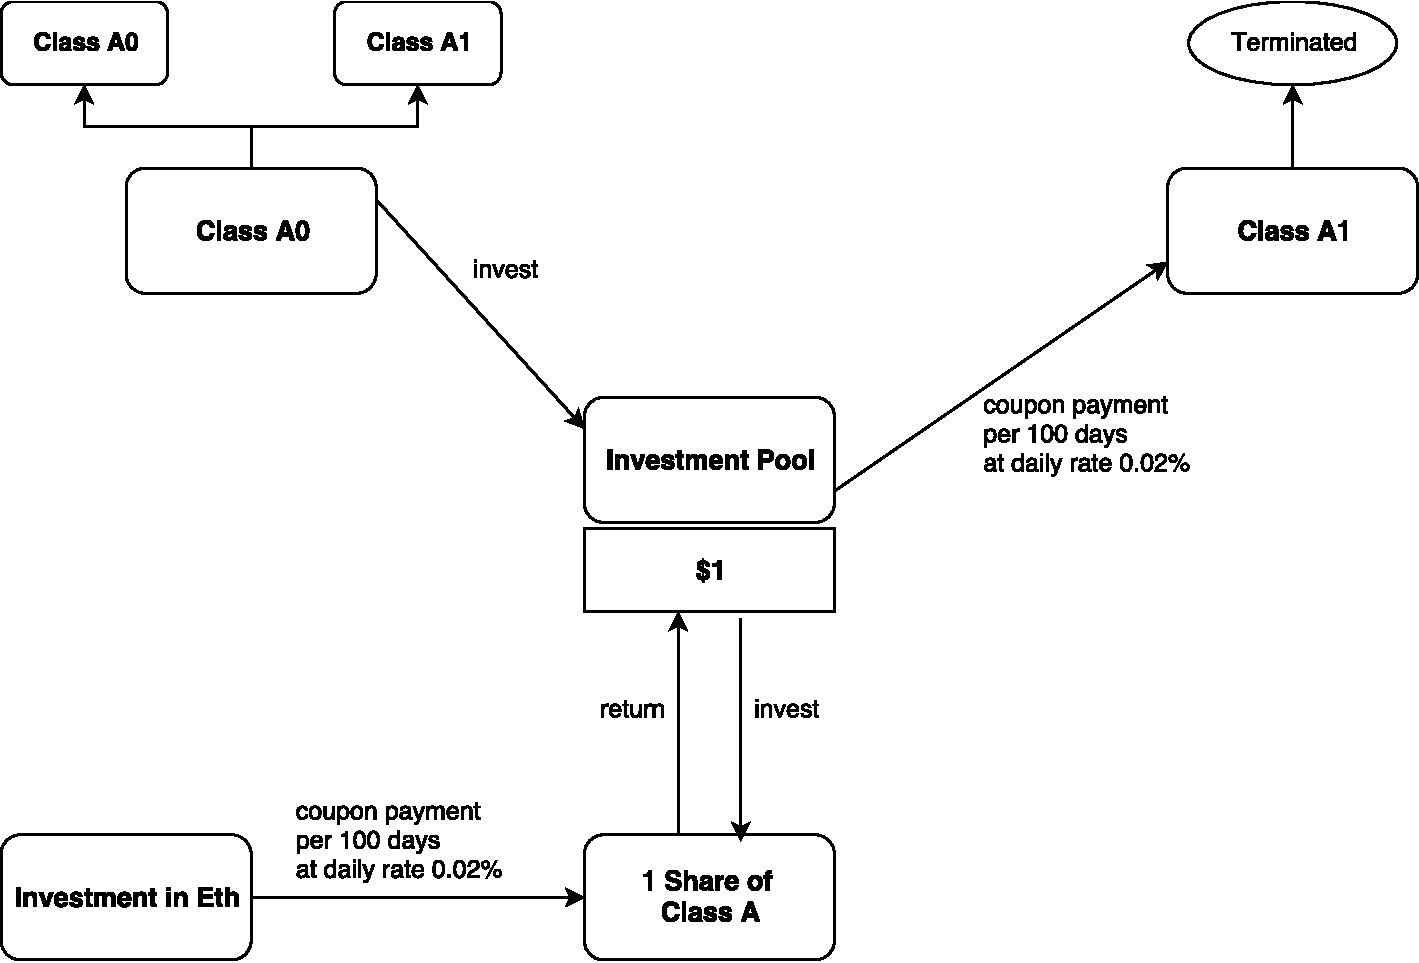
\includegraphics[width=0.8\textwidth]{A0_periodic.pdf}
\caption{\footnotesize  Class A0 receives no coupon.  Class A1 receives all the coupon payment. After the coupon payment, Class A1 is terminated, and 1 Class A0 is split into 1 new Class A0 and Class A1.}
\end{figure}

\end{frame}

\begin{frame}{A0 Coin, Upward Reset}

\begin{figure}
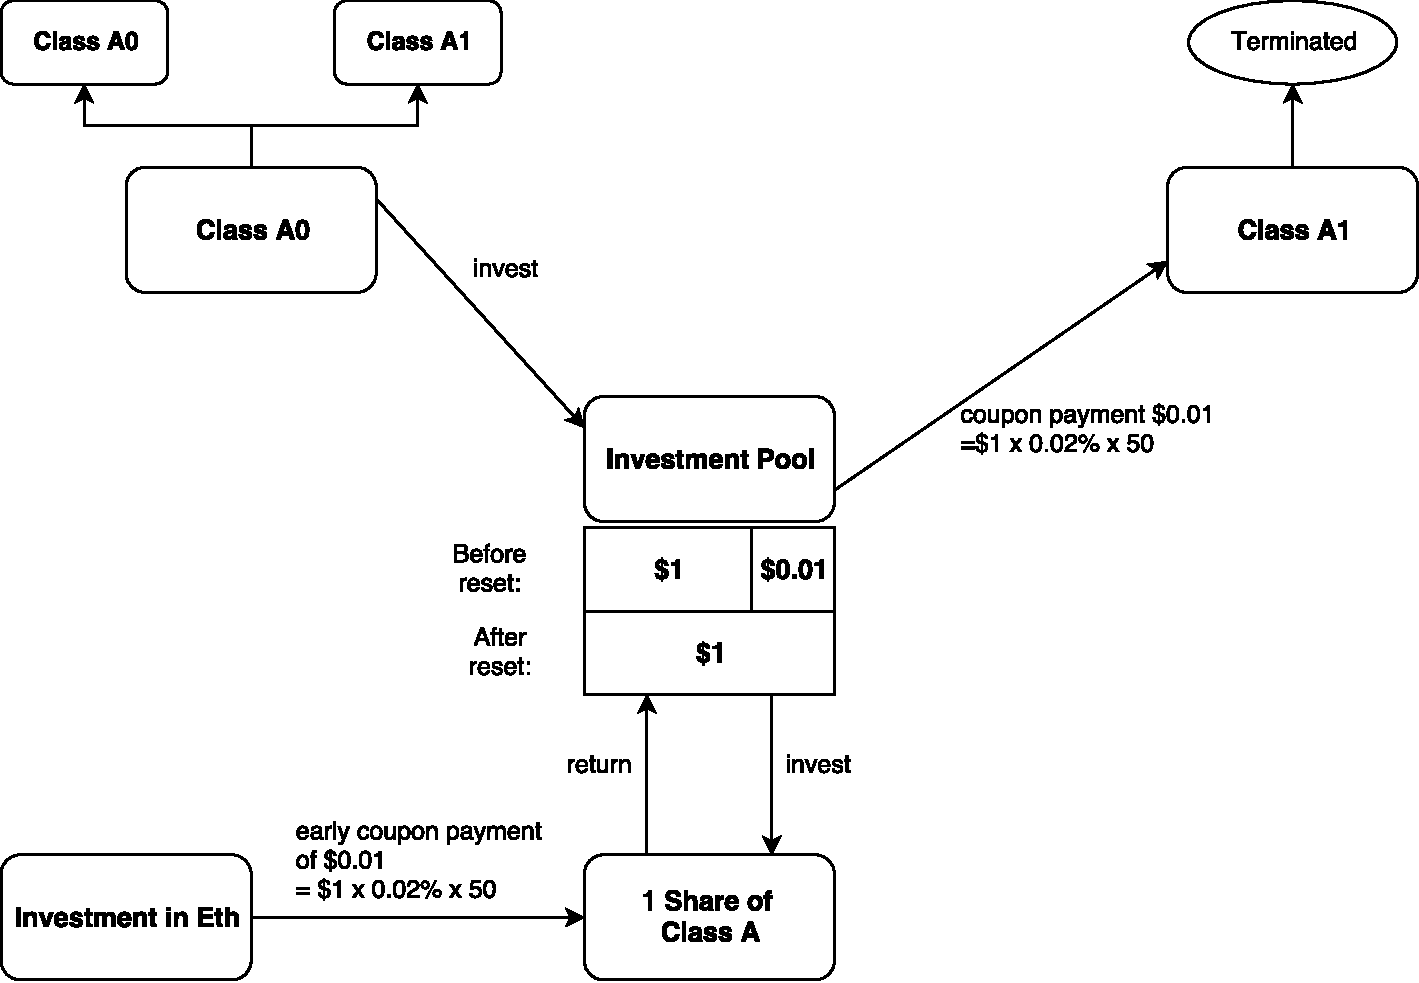
\includegraphics[width=0.7\textwidth]{A0_upward.pdf}
\caption{\footnotesize Upward Reset of Class A0. After 50 days, Class B NAV grows to \$2, triggering an upward reset.}
\end{figure}

\end{frame}


\begin{frame}{A0 Coin, Downward Reset}

\begin{figure}
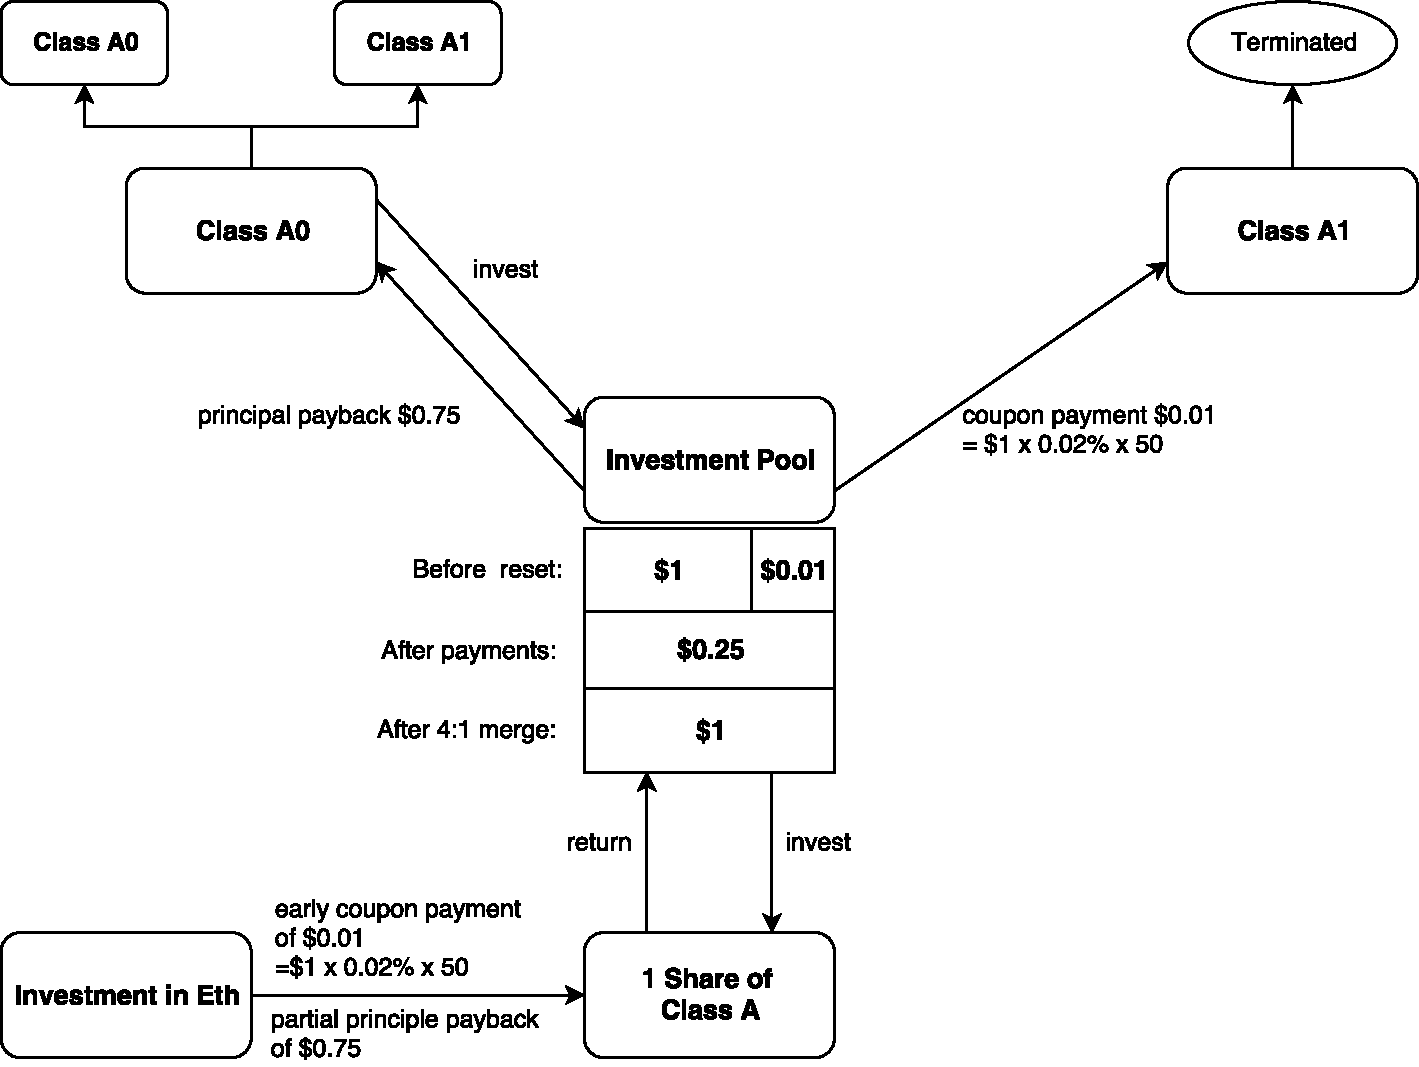
\includegraphics[width=0.78\textwidth]{A0_downward.pdf}
\caption{\footnotesize After another 50 days, Class B NAV drops to \$0.25, triggering a downward reset.}
\end{figure}


\end{frame}




\section{Valuation}

\begin{frame}{The Vanilla A and B Coins, Overview}

\begin{itemize}



\item
Let the downward reset boundary be $H_{d}(t)=\frac{1}{2}(1+Rt)+\frac{1}{2}\mathcal{H}_{d}$, and upward reset boundary $H_{u}(t)=\frac{1}{2}(1+Rt)+\frac{1}{2}\mathcal{H}_{u}$.

\item We have both stochastic representation and PDE for vanilla A and B coins.
\end{itemize}

\end{frame}


\begin{frame}{The Vanilla A and B Coins, Stochastic Representation}
\small
\begin{itemize}
\item $W_{A}(t,S)$ denotes the market value of Class A coin with time from last interest payment $0\le t\le T$, with $S_t=P_t/(\beta_t P_0)$, $H_{d}(t)\le S_t \le H_{u}(t)$.
\item $W_{A}(t,S)$ is given recursively by
\begin{align*}
\begin{split} ~ & E_{t}\Bigg[\sum_{1\le i<\tau\land\eta}e^{-r(i-t)}RT+e^{-r(\tau-t)}(R\tau+W_{A}(0,1))\cdot\mathbf{1}_{\{\tau<\eta\}}\\
 & \quad+e^{-r(\eta-t)}(R\eta+1-|V_{B}^{\eta-}|+(V_{B}^{\eta-})^+W_{A}(0,1))\cdot\mathbf{1}_{\{\eta<\tau\}}\Bigg],
\end{split}
\end{align*}
where $E_{t}$ is the expectation computed under the risk-neutral measure and under the initial condition $S_{t-}=S$,
\item The random times $\zeta$, $\tau$ and $\eta$ represent the first regular payout, upward and downward reset date from $t$, respectively. 

%On downward reset, if $V_B^{\eta-}>0$, A receives coupon, $1-V_B^{\eta-}$ shares of A is liquidated, and A receives the liquidation value; if $V_B^{\eta-}\le 0$, A is fully liquidated, and takes a loss by receiving $1+R\eta+V_B^{\eta-}$ which is smaller than the NAV $1+R\eta$.

\item Once we calculate $W_A$, the value of Class B coin can be calculated as $W_B=2S- W_A$.
\end{itemize}


\end{frame}

\begin{frame}{The Vanilla A and B Coins, PDE}

We assume that $P_t$ follows a geometric Brownian motion under the risk neutral measure:
\begin{align*}
dP_{t}=r P_tdt+\sigma P_{t}dW_{t},
\end{align*}
where $W_{t}$ is a one-dimensional standard Brownian motion.




$W_{A}(t,S)$ is the unique solution of the following periodic PDE with nonlocal boundary and nonlocal terminal conditions, 
\begin{align*}
-\frac{\partial W_{A}}{\partial t} & =\frac{1}{2}\sigma^{2}S^{2}\frac{\partial^{2}W_{A}}{\partial S^{2}}+r S\frac{\partial W_{A}}{\partial S}-r W_{A}, \\
&   ~~t\in[0,T),~S\in (H_d(t),H_u(t))\\
W_{A}(T,S) & =RT+W_{A}(0,S-\frac{1}{2}RT),\\
W_{A}(t,H_{u}(t)) & =Rt+W_{A}(0,1)\\
W_{A}(t,H_d(t)) & =Rt+1-\mathcal{H}_{d}+\mathcal{H}_{d}W_{A}(0,1).
\end{align*}



\end{frame}

\begin{frame}{The  A' and B' Coins, Stochastic Representation}
\small
Under the risk-neutral pricing framework, the value $W_{A^\prime}(t,S)$ of Class A' is given as
{\scriptsize\begin{align*}
\begin{split} ~& E_{t}\Bigg[\sum_{1\le i<\tau\land\eta}e^{-r(i-t)}R^\prime T+e^{-r(\tau-t)}(R^\prime\tau+W_{A^\prime}(0,1))\cdot\mathbf{1}_{\{\tau<\eta\}}\\
 & \quad+e^{-r(\eta-t)}\left(\min\{R^\prime\eta+1-(V_{B}^{\eta-})^+,2(R\eta+1+V_B^{\eta-})^+\}+(V_{B}^{\eta-})^+W_{A^\prime}(0,1)\right)\cdot\mathbf{1}_{\{\eta<\tau\}}\Bigg],
\end{split}
\end{align*}}
where $\tau$ and $\eta$ are the first upward and downward reset of Class A (or equivalently, Class A' and B') after $t$, respectively. On downward reset, if $V_B^{\eta-}>0$, A receives coupon $R^\prime\eta$, $1-V_B^{\eta-}$ shares of A is liquidated, and A receives the liquidation value; if $\frac{R^\prime\eta-1}{2}-R\eta\le V_B^{\eta-}\le 0$, A is fully liquidated, and still receives full NAV; otherwise, A is fully liquidated and takes a loss by receiving $2(1+R\eta+V_B^{\eta-})^+$ which is smaller than the NAV $1+R\eta$.
\end{frame}


\begin{frame}{The A' and B' Coins, PDE}


We assume that $P_t$ follows a geometric Brownian motion.





$W_{A^\prime}$ satisfies the following PDE, which is the same as that for $W_{A}$, except changing $R$ to $R^\prime$ for the coupon payment:
\begin{align*}
-\frac{\partial W_{A^\prime}}{\partial t} & =\frac{1}{2}\sigma^{2}S^{2}\frac{\partial^{2}W_{A^\prime}}{\partial S^{2}}
   +r S\frac{\partial W_{A^\prime}}{\partial S}-r W_{A^\prime}, \\
   &~~t\in[0,T),~S\in (H_d(t),H_u(t))\\
W_{A^\prime}(T,S) & =R^\prime T+W_{A^\prime}(0,S-\frac{1}{2}RT),\\
W_{A^\prime}(t,H_{u}(t)) & =R^\prime t+W_{A^\prime}(0,1)\\
W_{A^\prime}(t,H_d(t)) & =R^\prime t+1-\mathcal{H}_{d}+\mathcal{H}_{d}W_{A^\prime}(0,1).
\end{align*}
\end{frame}

\begin{frame}{The  A0 and A1 Coins, Stochastic Representation}

Under the risk-neutral pricing framework, the market value $W_{A1}(t,S)$ of Class A1 coin is given as
\begin{align*}
 & E_{t}\Bigg[e^{-r(\zeta-t)}RT\cdot\mathbf{1}_{\{\zeta\le\tau,\eta\}}+e^{-r(\tau-t)}R\tau\cdot\mathbf{1}_{\{\tau<\eta,\zeta\}}\\
 &\quad+e^{-r(\eta-t)}(R\eta-(V_B^{\eta-})^-)^+\cdot\mathbf{1}_{\{\eta<\tau,\zeta\}}\Bigg],
\end{align*}
where the first regular payout time $\zeta$, the first upward reset time $\tau$ and the first downward reset time $\eta$ are defined as before. On a downward reset, if $V_B^{\eta-}>0$, A1 gets the coupon payment $R\eta$; if $V_B^{\eta-}\le 0$, A1 only gets a part of the coupon $(R\eta+V_B^{\eta-})^+ < R\eta$. 


\end{frame}


\begin{frame}{The A0 and A1 Coins, PDE}

We assume that $P_t$ follows a geometric Brownian motion.

$W_{A1}$ is the unique solution of the following PDE
\begin{align*}
-\frac{\partial W_{A1}}{\partial t} & =\frac{1}{2}\sigma^{2}S^{2}\frac{\partial^{2}W_{A1}}{\partial S^{2}}+r S\frac{\partial W_{A1}}{\partial S}-r W_{A1},\\
& ~~t\in[0,T),~S\in (H_d(t),H_u(t))\\
W_{A1}(T,S) & =RT\\
W_{A1}(t,H_{u}(t)) & =Rt\\
W_{A1}(t,H_d(t)) & =Rt.
\end{align*}
Finally, the value of Class A0 coin is defined as $W_{A0}=W_A-W_{A1}$.

\end{frame}


\section{Numerical Examples}


\begin{frame}{The Setting}

For illustration, we hereby uses Ether (ETH) as the underlying coin
and apply below parameter values:
\begin{align*}
R& =0.02\% \text{ (7.3\% p.a.)} & R^\prime & = 0.0082\% \text{ (3\% p.a.)}\\
\mathcal{H}_{u} & =2 & \mathcal{H}_{p} & =1.02\\
\mathcal{H}_{d} & =0.25 & T &= 100\\
\sigma &= 0.0628 \text{ (120\% p.a.)} & r&=0.0082\% \text{ (3\% p.a.)}.
\end{align*}
The following assumptions are used:
\begin{enumerate}
\item Price is monitored on daily basis
\item Resets are performed according to end-of-day prices
\item Reinvestment of ETH payout from resets is not considered
\end{enumerate}

\end{frame}



\begin{frame}{Class A, Simulated Market Values}

\begin{figure}[htb]
\begin{centering}
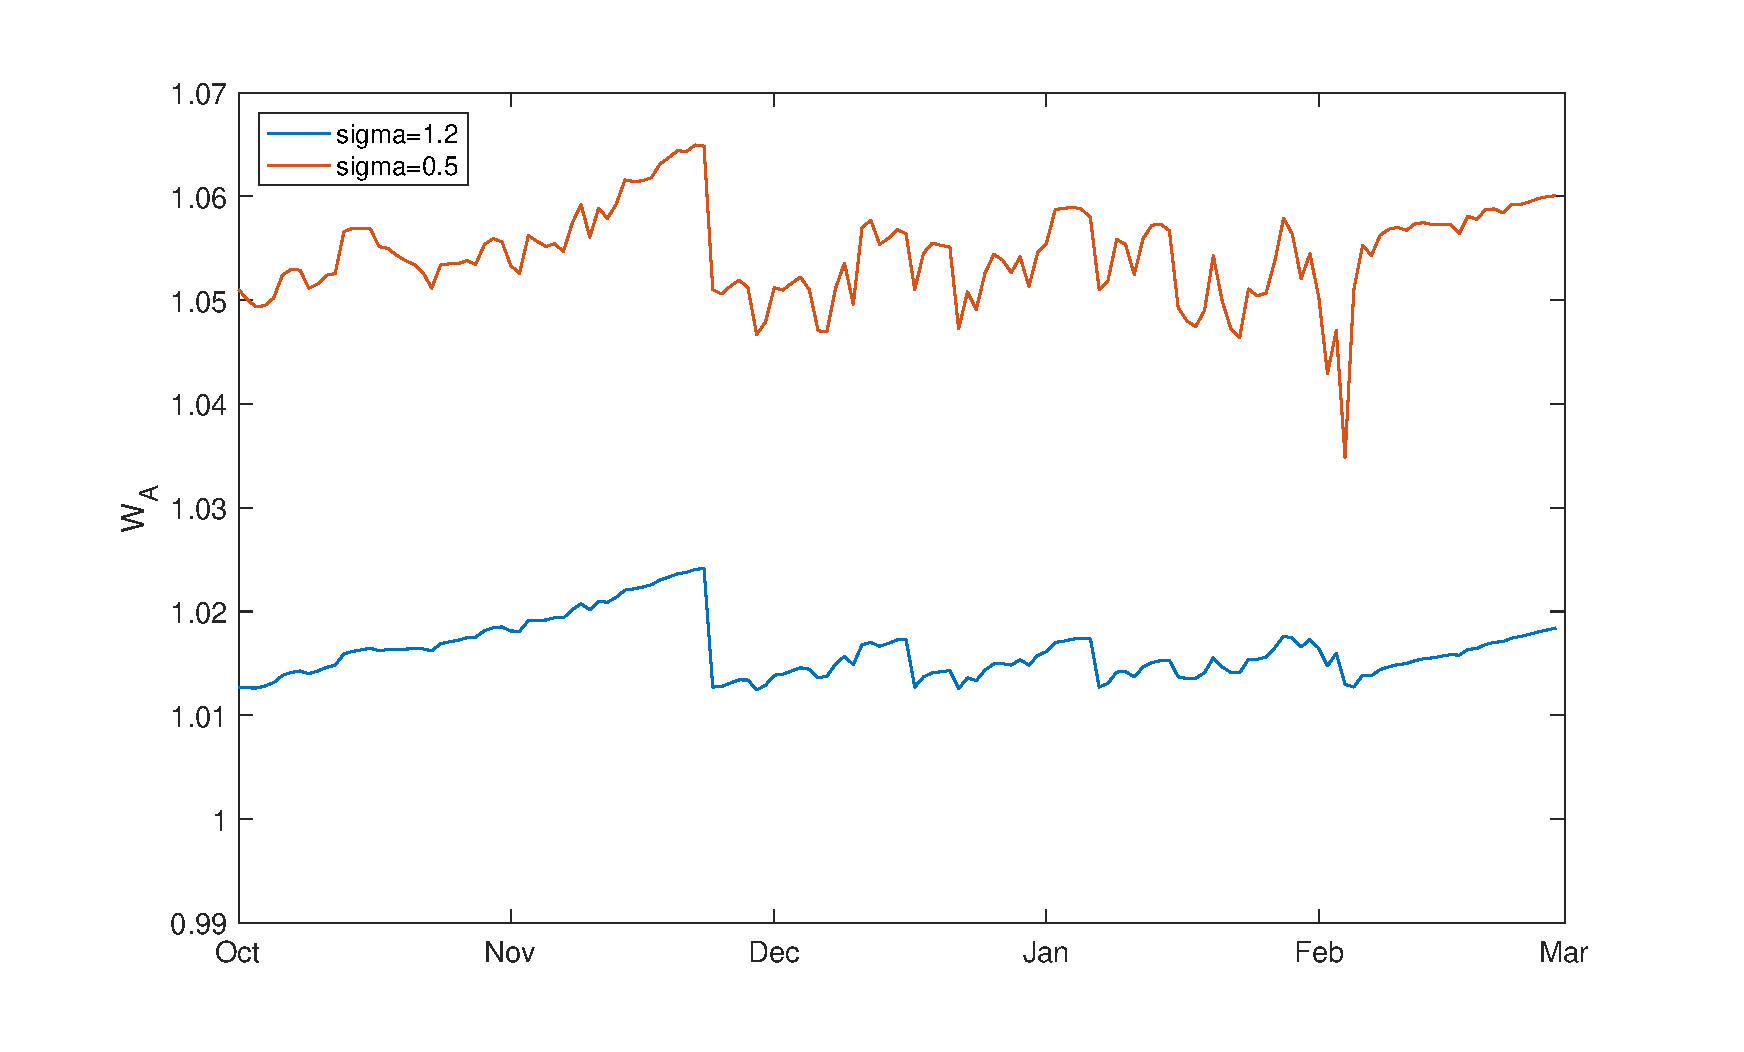
\includegraphics[width=0.85\textwidth]{WA.eps}
\par\end{centering}
\caption{Simulated class A Market Value.  Upward reset takes place on 24 Nov 2017, 17 Dec 2017, and 7 Jan 2018. Downward reset date takes place on 5 Feb 2018.}\label{fig:valA}
\end{figure}

\end{frame}

\begin{frame}{Class B, Simulated Market Values}


\begin{figure}[htb]
\begin{centering}
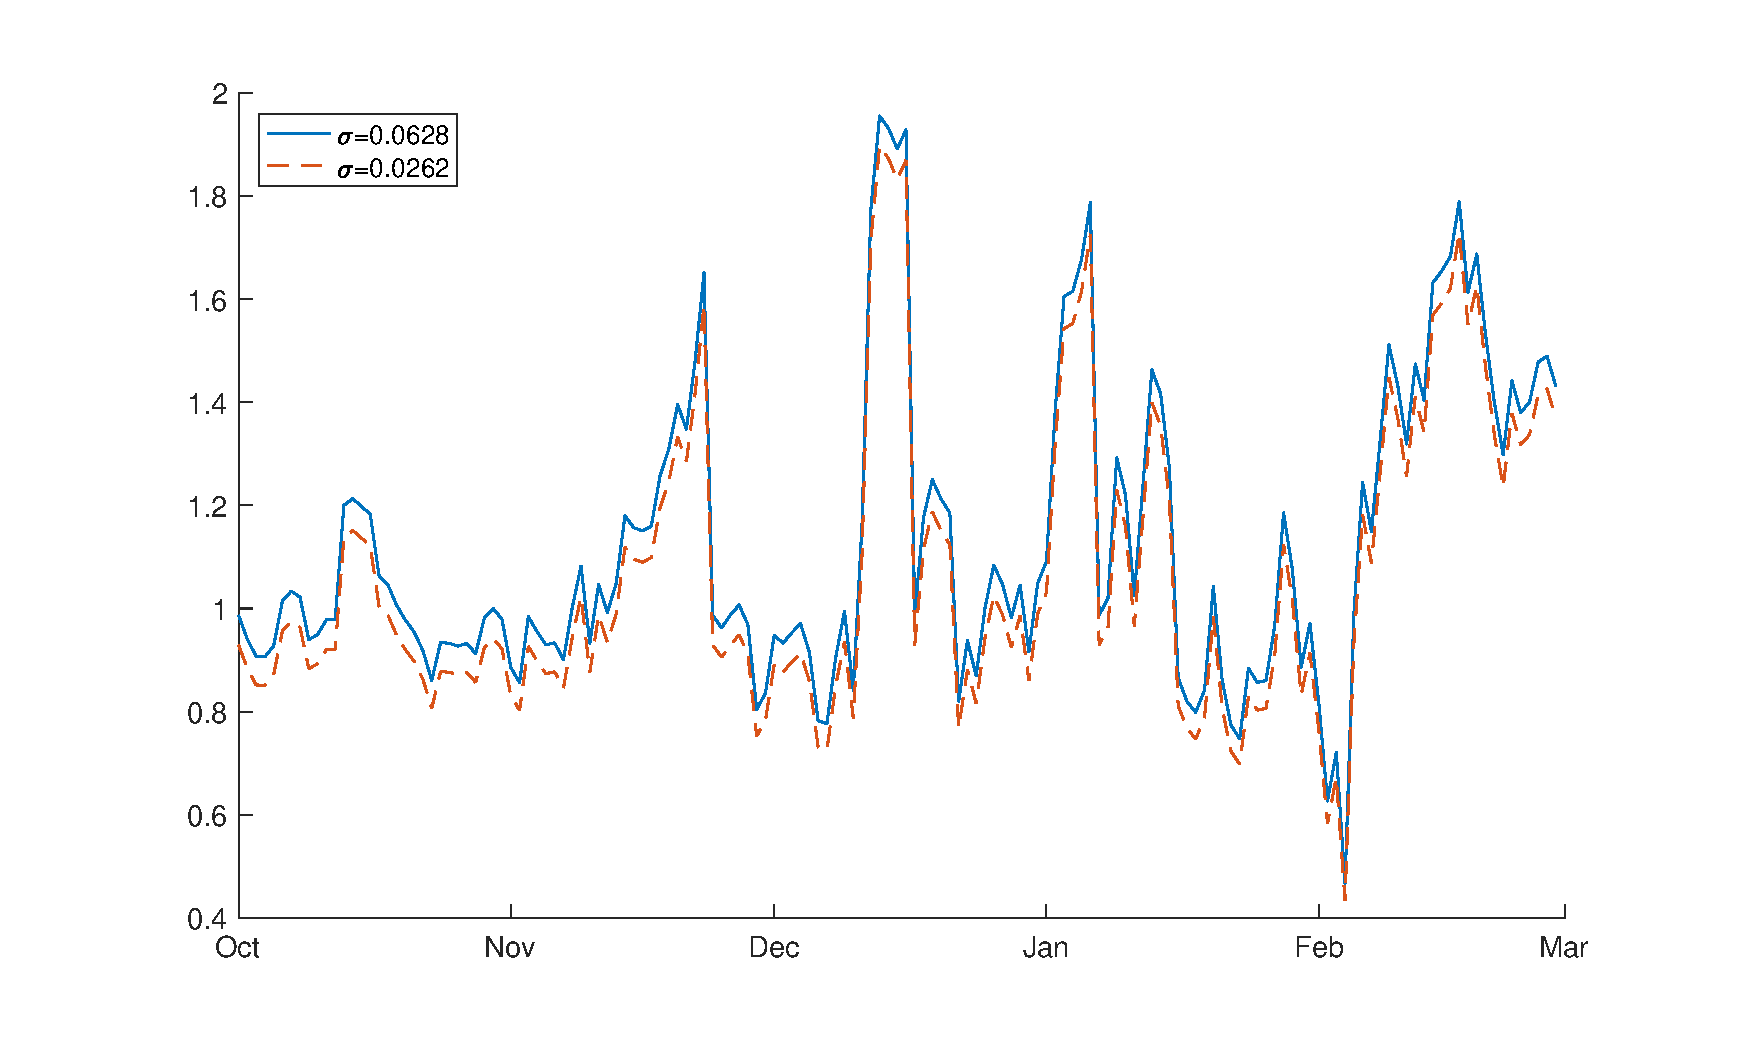
\includegraphics[width=0.85\textwidth]{WB}
\par\end{centering}
\caption{Class B Market Value. B has upward resets (on 24 Nov 2017, 17 Dec 2017, and 7 Jan 2018) with dividend payments \$1.0846, \$1.0467, and \$1.1106 and downward resets on 5 Feb, 2018. }
\label{fig:valB}
\end{figure}
\end{frame}


\begin{frame}{Class A', Simulated Market Values}



\begin{figure}[htb]
\centering
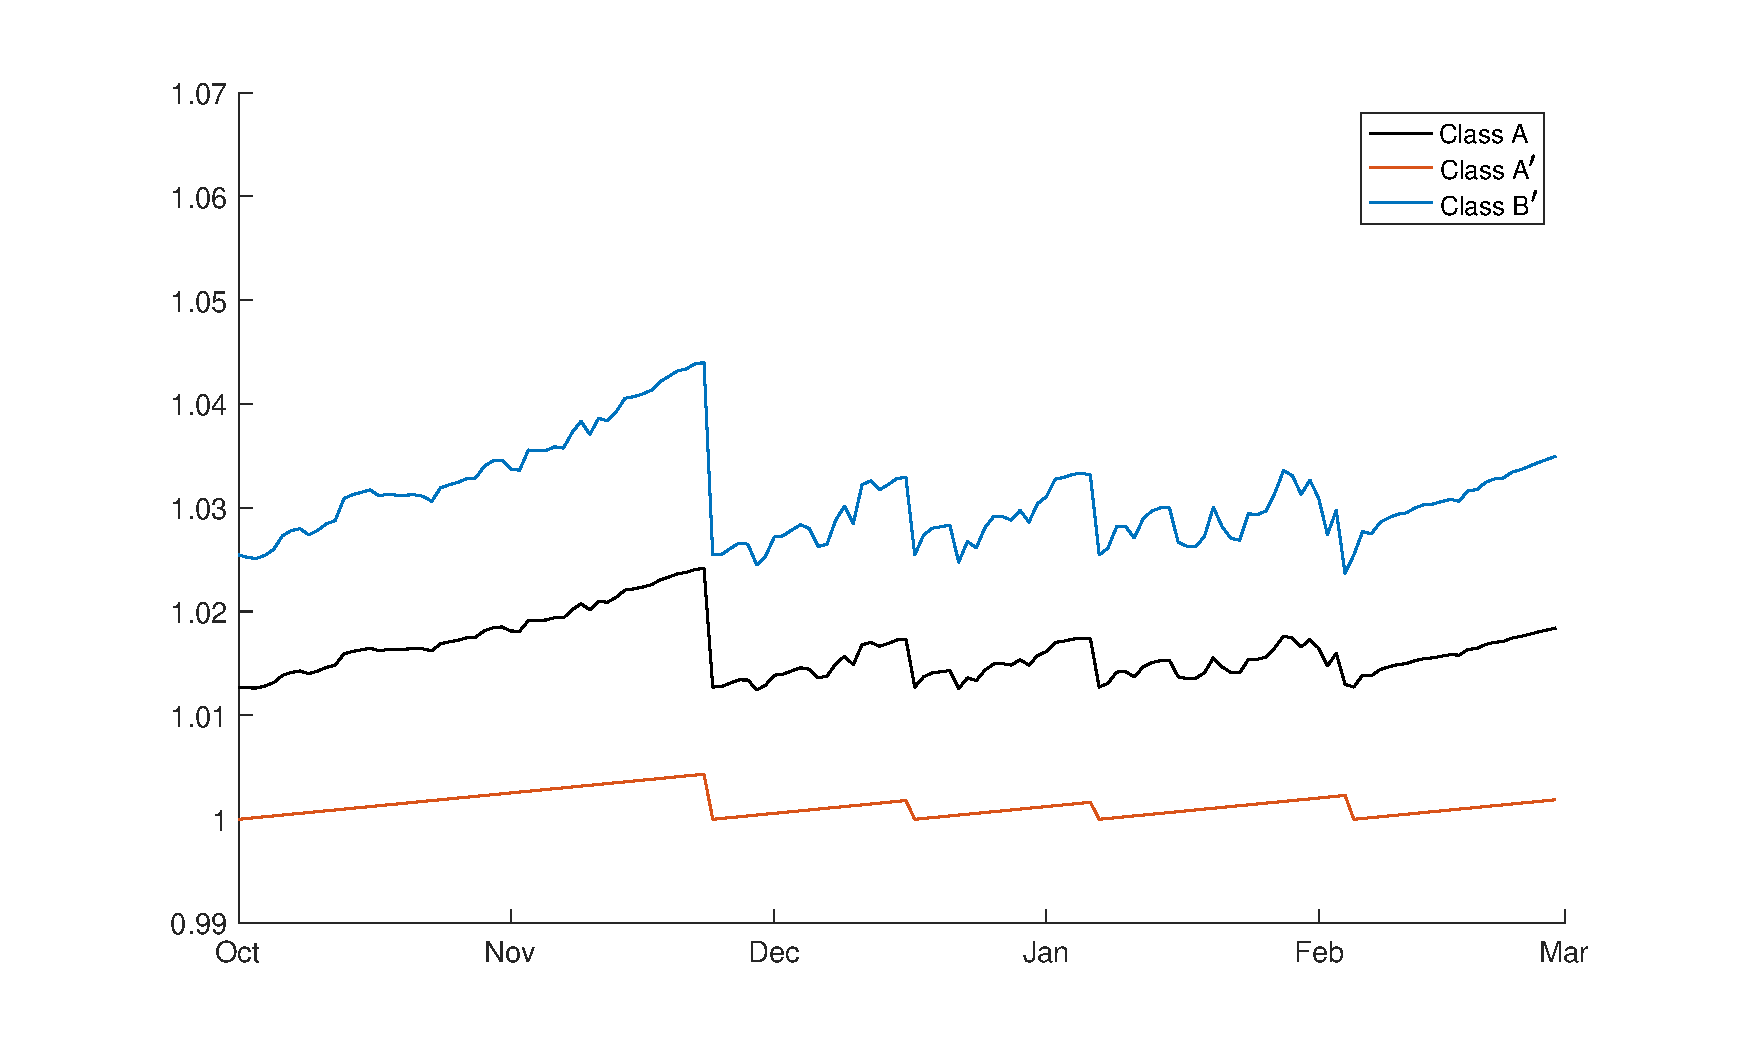
\includegraphics[width=0.95\textwidth]{WABpnoCI4.eps}
\caption{Market Value of Class A$^\prime$ (red) and B$^\prime$ (yellow), compared with Class A (blue).}
\label{fig:valAPrime}
\end{figure}

\end{frame}

\begin{frame}{Class A', Simulated Market Values}

\begin{itemize}
\item The 4 downward jumps correspond to the coupon payment of Class A' on 1 downward and 3 upward reset dates of Class A.
\item If we de-trend the value of Class A$^\prime$ by its NAV and consider $W_{A^\prime}-V_{A^\prime}$, it has an annualized standard deviation of $5.4\times 10^{-5}$, which is much smaller than that of $W_{A}-V_{A}$ (0.0178).
\end{itemize}

\end{frame}

\begin{frame}{Class A0, Simulated Market Values, 1:1 Split}




\begin{figure}[htb]
\centering
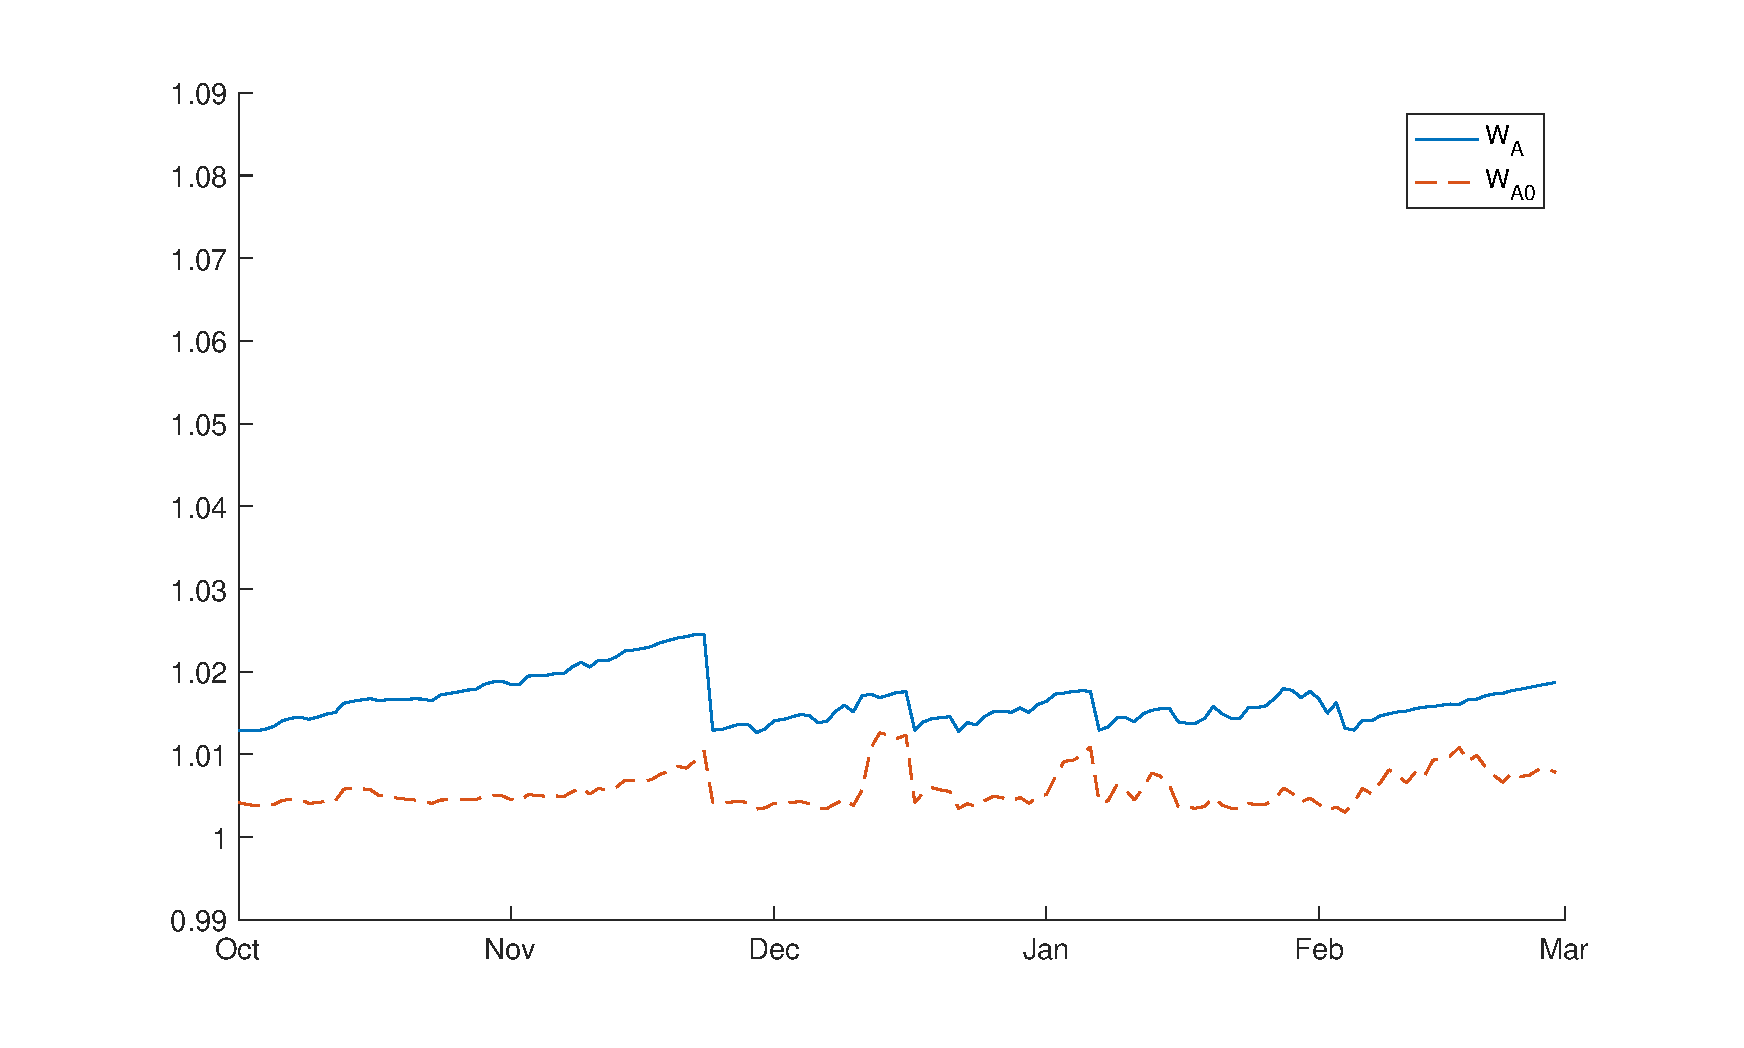
\includegraphics[width=0.95\textwidth]{WA0_alpha1.eps}
\caption{Market Value of Class A0 compared to Class A. }
\label{fig:valA0a1}
\end{figure}
\end{frame}

\begin{frame}{Class A0, Simulated Market Values, 2:1 Split}

\begin{figure}[htb]
\centering
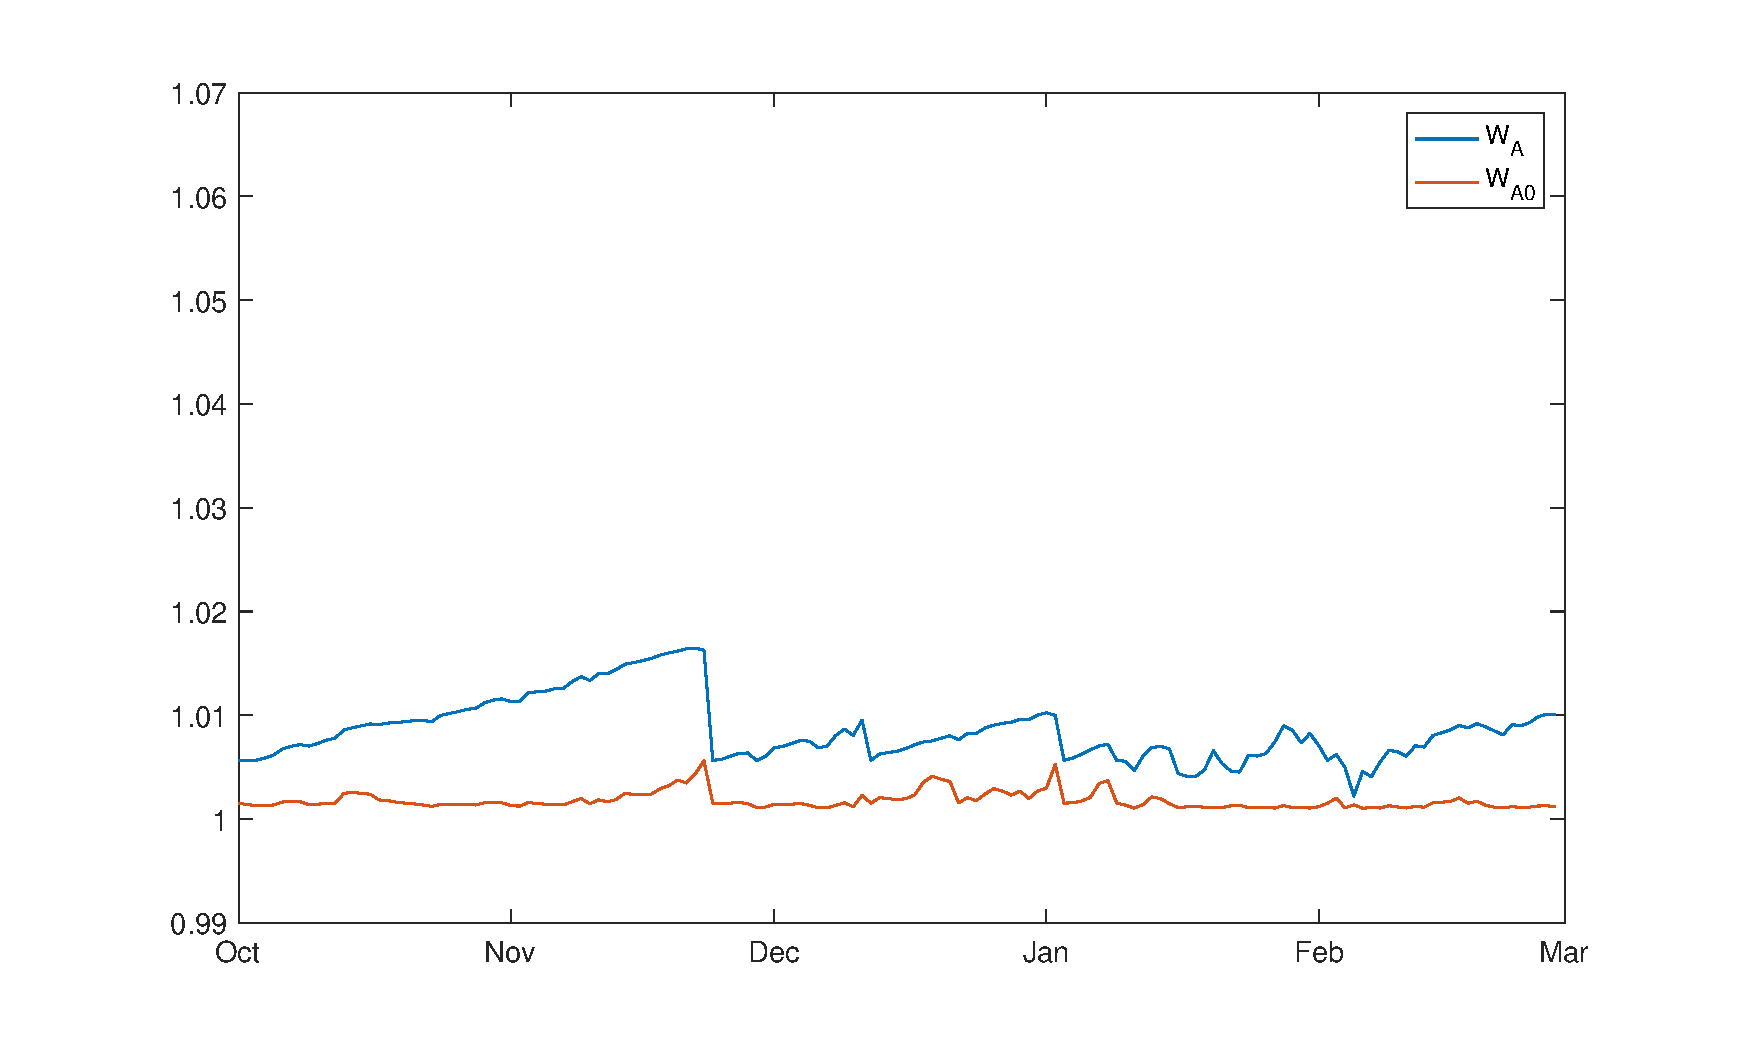
\includegraphics[width=0.95\textwidth]{WA0_alpha2.eps}
\caption{Market Value of Class A0 (principal only class) compared to Class A.}
\label{fig:valA0a2}
\end{figure}
\end{frame}


\begin{frame}{Class A0, Simulated Market Values}

\begin{itemize}
\item The 4 downward jumps correspond to the coupon payment of Class A0 on 1 downward and 3 upward reset dates of Class A.
\item A0 has an annualized standard deviation of $0.0413$ for $\alpha=1$, 
as compared to SD of $W_{A}$, which is 0.0530.
\item A0 has an annualized standard deviation of $0.0156$ for $\alpha=2$, 
as compared to SD of $W_{A}$, which is 0.0571. Note that with $\alpha=2$, the NAV of B is $3S_t -2(1+Rt)$, making B more sensitive to $S_t$.
\end{itemize}
\end{frame}




\begin{frame}{Black Swan Events}
\begin{itemize}
  \item Let us assume that if an extreme event happens, then there is a 80\% sudden drop in the Eth price.
  \item Assuming $\beta=1$, $P_{t-}=P_0=500$ (so that the relative price $S_{t-}=1$), and $P$ suddenly drops to $P_t=100$.
  \item Then the NAV of Class A coins $V_A^t=2\times S_{t-}\times(1-80\%)=0.4$, while the NAV of Class A$^\prime$ coins $V_{A^\prime}^t=2\times V_A^t=0.8$.
  \item Assuming that this kind of downward jump occurs in a jump diffusion model with a Poisson intensity 0.2 per year and constant jump size $-80\%$, then we have at time 0,  $W_A (0) =0.888$ and $W_{A^\prime} (0) =0.962$; in contrast, if there is no jump risk (intensity equals 0), $W_A (0) =1.013$, $W_{A^\prime} (0) =1.000$. 
  \item Therefore, the presence of extreme jump risk has a smaller impact on Class A$^\prime$ coins.
\end{itemize}
\end{frame}




\section{Conclusion}


\begin{frame}{Conclusion}

\begin{itemize}
\item Within the ecology system of Blockchains, stable coins are needed to settle transactions, to pay miners, and to do asset allocation.
\item We design several classes of stable coins, A' and A0, based on vanilla A, which are inspired by the dual purpose funds in China and U.S.
\item These stable coins can be used as a basis for sovereign stable coins, if a government can provide the insurance in extreme events.
\end{itemize}

\end{frame}


\begin{frame}{}
\begin{center}
{\LARGE Thank you.}
\end{center}
\end{frame}



\end{document}
